% Section 3.8: Orchestration System Design
\clearpage
\section{3.8 Orchestration System Design}
\label{sec:orchestration-system}
\addcontentsline{toc}{section}{3.8 Orchestration System Design}

\lettrine{T}{his section} explores Symphony's orchestration system, the intelligence layer that coordinates multiple AI agents and tools to accomplish complex development tasks. We examine the Conductor's reinforcement learning approach, the Melody workflow abstraction, and the execution mechanisms that enable Agent-Driven Development. The orchestration system transforms high-level developer intent into concrete, executable workflows while continuously learning and improving from experience.

\subsection*{3.8.1 The Conductor and Reinforcement Learning}
\addcontentsline{toc}{subsection}{3.8.1 The Conductor and Reinforcement Learning}

The orchestration system represents the intelligence layer that enables Symphony to coordinate multiple AI agents and tools to accomplish complex development tasks. The orchestration philosophy embraces Agent-Driven Development, where specialized AI agents collaborate under intelligent coordination to handle implementation details while developers provide vision and strategic guidance.

The Conductor serves as the central intelligence within the orchestration system, implementing a reinforcement learning model that learns optimal workflow patterns from experience. The Conductor analyzes developer prompts to understand intent, examines project context, selects appropriate extensions and models for each task, determines execution sequence, and monitors execution for optimization opportunities. This intelligent coordination enables automatic workflow generation, significantly reducing cognitive load.

The system architecture consists of two main components that work together seamlessly:

\clearpage
\textbf{Component 1: IPC Communication Infrastructure}

The Conductor communicates with the core system through an inter-process communication infrastructure enabling seamless integration despite being implemented in Python while the core is in Rust. The IpcBus provides reliable message passing with Transport layer supporting Unix sockets (Linux/macOS) and named pipes (Windows). The Protocol layer handles message serialization and deserialization, ensuring safe data transmission between processes. The Security layer implements authentication and rate limiting to protect against malicious extensions. The Message component carries data with unique IDs, sender/receiver process IDs, payload bytes, and timestamps as illustrated in ~\ref{fig:3.17-ipc-infrastructure}.

\begin{figure}[H]
\centering
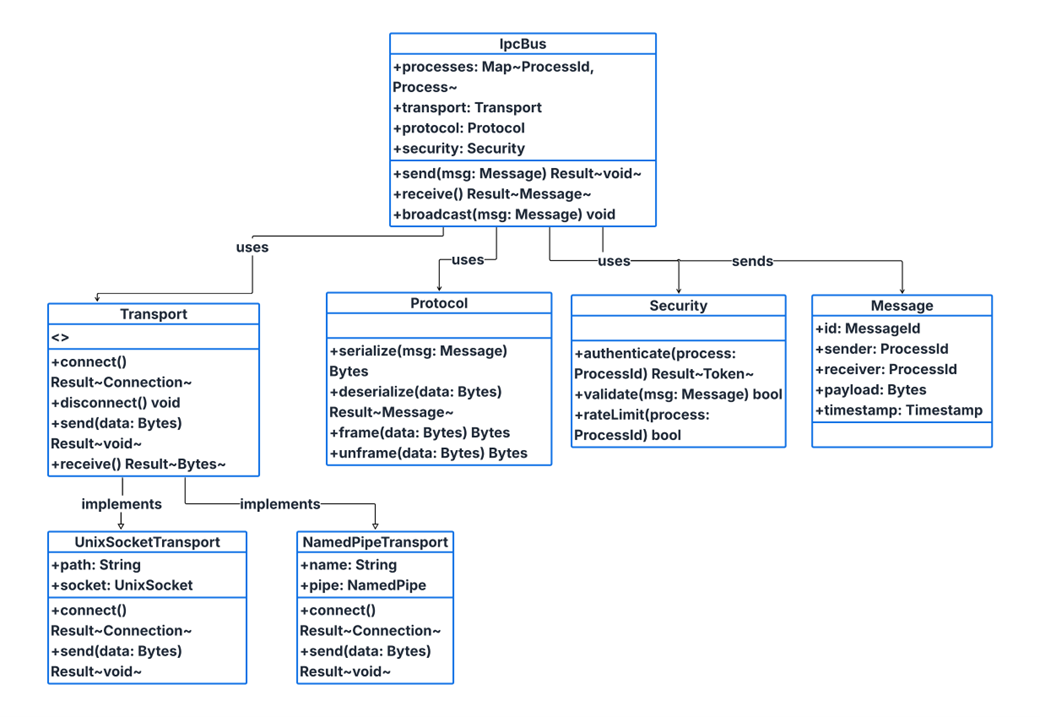
\includegraphics[width=1.20\textwidth]{images/diagrams/class_diagram/seperate_3_ipc_communication_conductor_rl/IPC Communication Infrastructure.png}
\caption{IPC Communication Infrastructure}
\label{fig:3.17-ipc-infrastructure}
\end{figure}

\clearpage
\textbf{Component 2: Conductor Architecture}

The Conductor component integrates the reinforcement learning model with the orchestration system. The RlModel implements the policy and value function, predicting actions from states and updating through experience. The OrchestrationBridge converts between Melody workflows and DAG structures, collecting execution rewards. The PyO3Bindings enable seamless Rust-Python interoperability, converting values between languages and calling Python functions from Rust. This architecture enables the Conductor to leverage Python's ML ecosystem while maintaining Rust core performance as illustrated in ~\ref{fig:3.18-conductor-architecture}.

\begin{figure}[H]
\centering
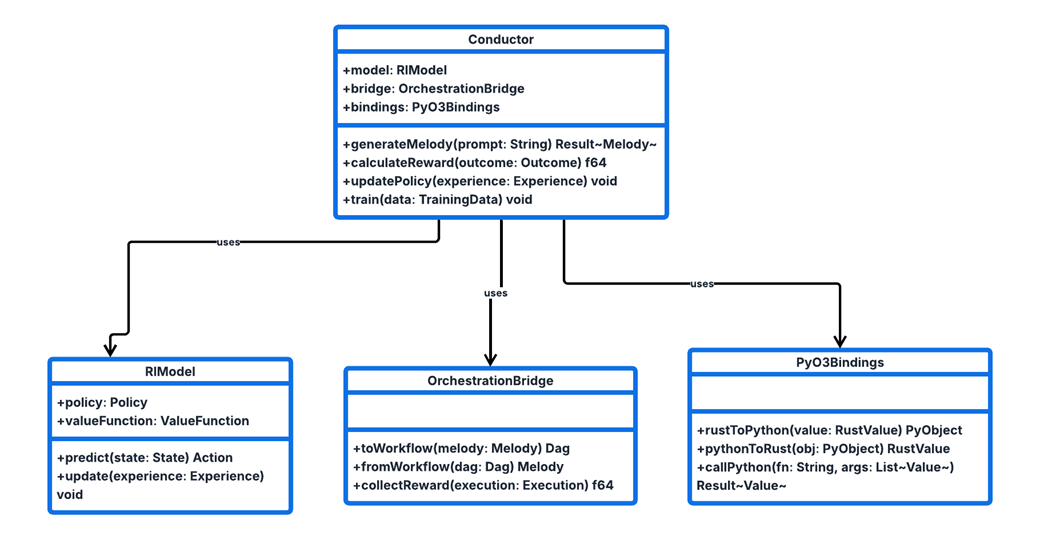
\includegraphics[width=1.20\textwidth]{images/diagrams/class_diagram/seperate_3_ipc_communication_conductor_rl/Conductor Architecture.png}
\caption{Conductor Architecture - RL Model and Integration Components}
\label{fig:3.18-conductor-architecture}
\end{figure}

\clearpage
The reinforcement learning model learns from every workflow execution, continuously improving its ability to generate effective task sequences. The model treats workflow generation as a sequential decision problem, selecting the next task based on current state. The state representation includes developer prompt, project context, existing workflow tasks, and available extensions. The model outputs a probability distribution over possible next tasks, sampling to generate diverse workflows.

The reward signal drives learning from multiple sources: execution success (objective accomplishment), execution time (efficiency), artifact quality (output value), and user feedback (developer satisfaction). These components combine into a single scalar value guiding the learning process. The model updates parameters after each execution using policy gradient methods, increasing probability of high-reward actions and decreasing probability of low-reward actions.


% \clearpage
\subsection*{3.8.2 Melody System and Workflow Generation}
\addcontentsline{toc}{subsection}{3.8.2 Melody System and Workflow Generation}

The Melody concept provides the abstraction through which developers interact with workflows in Symphony. A Melody represents a complete workflow as a directed acyclic graph where nodes represent individual tasks and edges represent dependencies between tasks. Melodies can be created manually through the visual Harmony Board interface or generated automatically by the Conductor based on natural language prompts. Once created, Melodies can be saved, shared, and reused, building up a library of proven workflows for common development tasks. The Melody abstraction enables developers to think about workflows at a high level without concerning themselves with the details of how individual tasks are implemented or coordinated.

The execution of a Melody involves multiple system components working together in a coordinated fashion, which can be understood through three distinct phases:

\clearpage
\textbf{Phase 1: Orchestration Flow}

The workflow begins when the developer writes a prompt describing the desired outcome. The Frontend UI submits this prompt to the Core system, which forwards it to the Conductor for processing. The Conductor analyzes the prompt and generates a Melody workflow. In Maestro Mode, the Conductor uses reinforcement learning to automatically generate the workflow. In Manual Mode, the system requests the developer to select from available Melodies through a browser interface. Once the Melody is selected or generated, the Conductor orchestrates its execution as illustrated in ~\ref{fig:3.19-melody-orchestration}.

\begin{figure}[H]
\centering
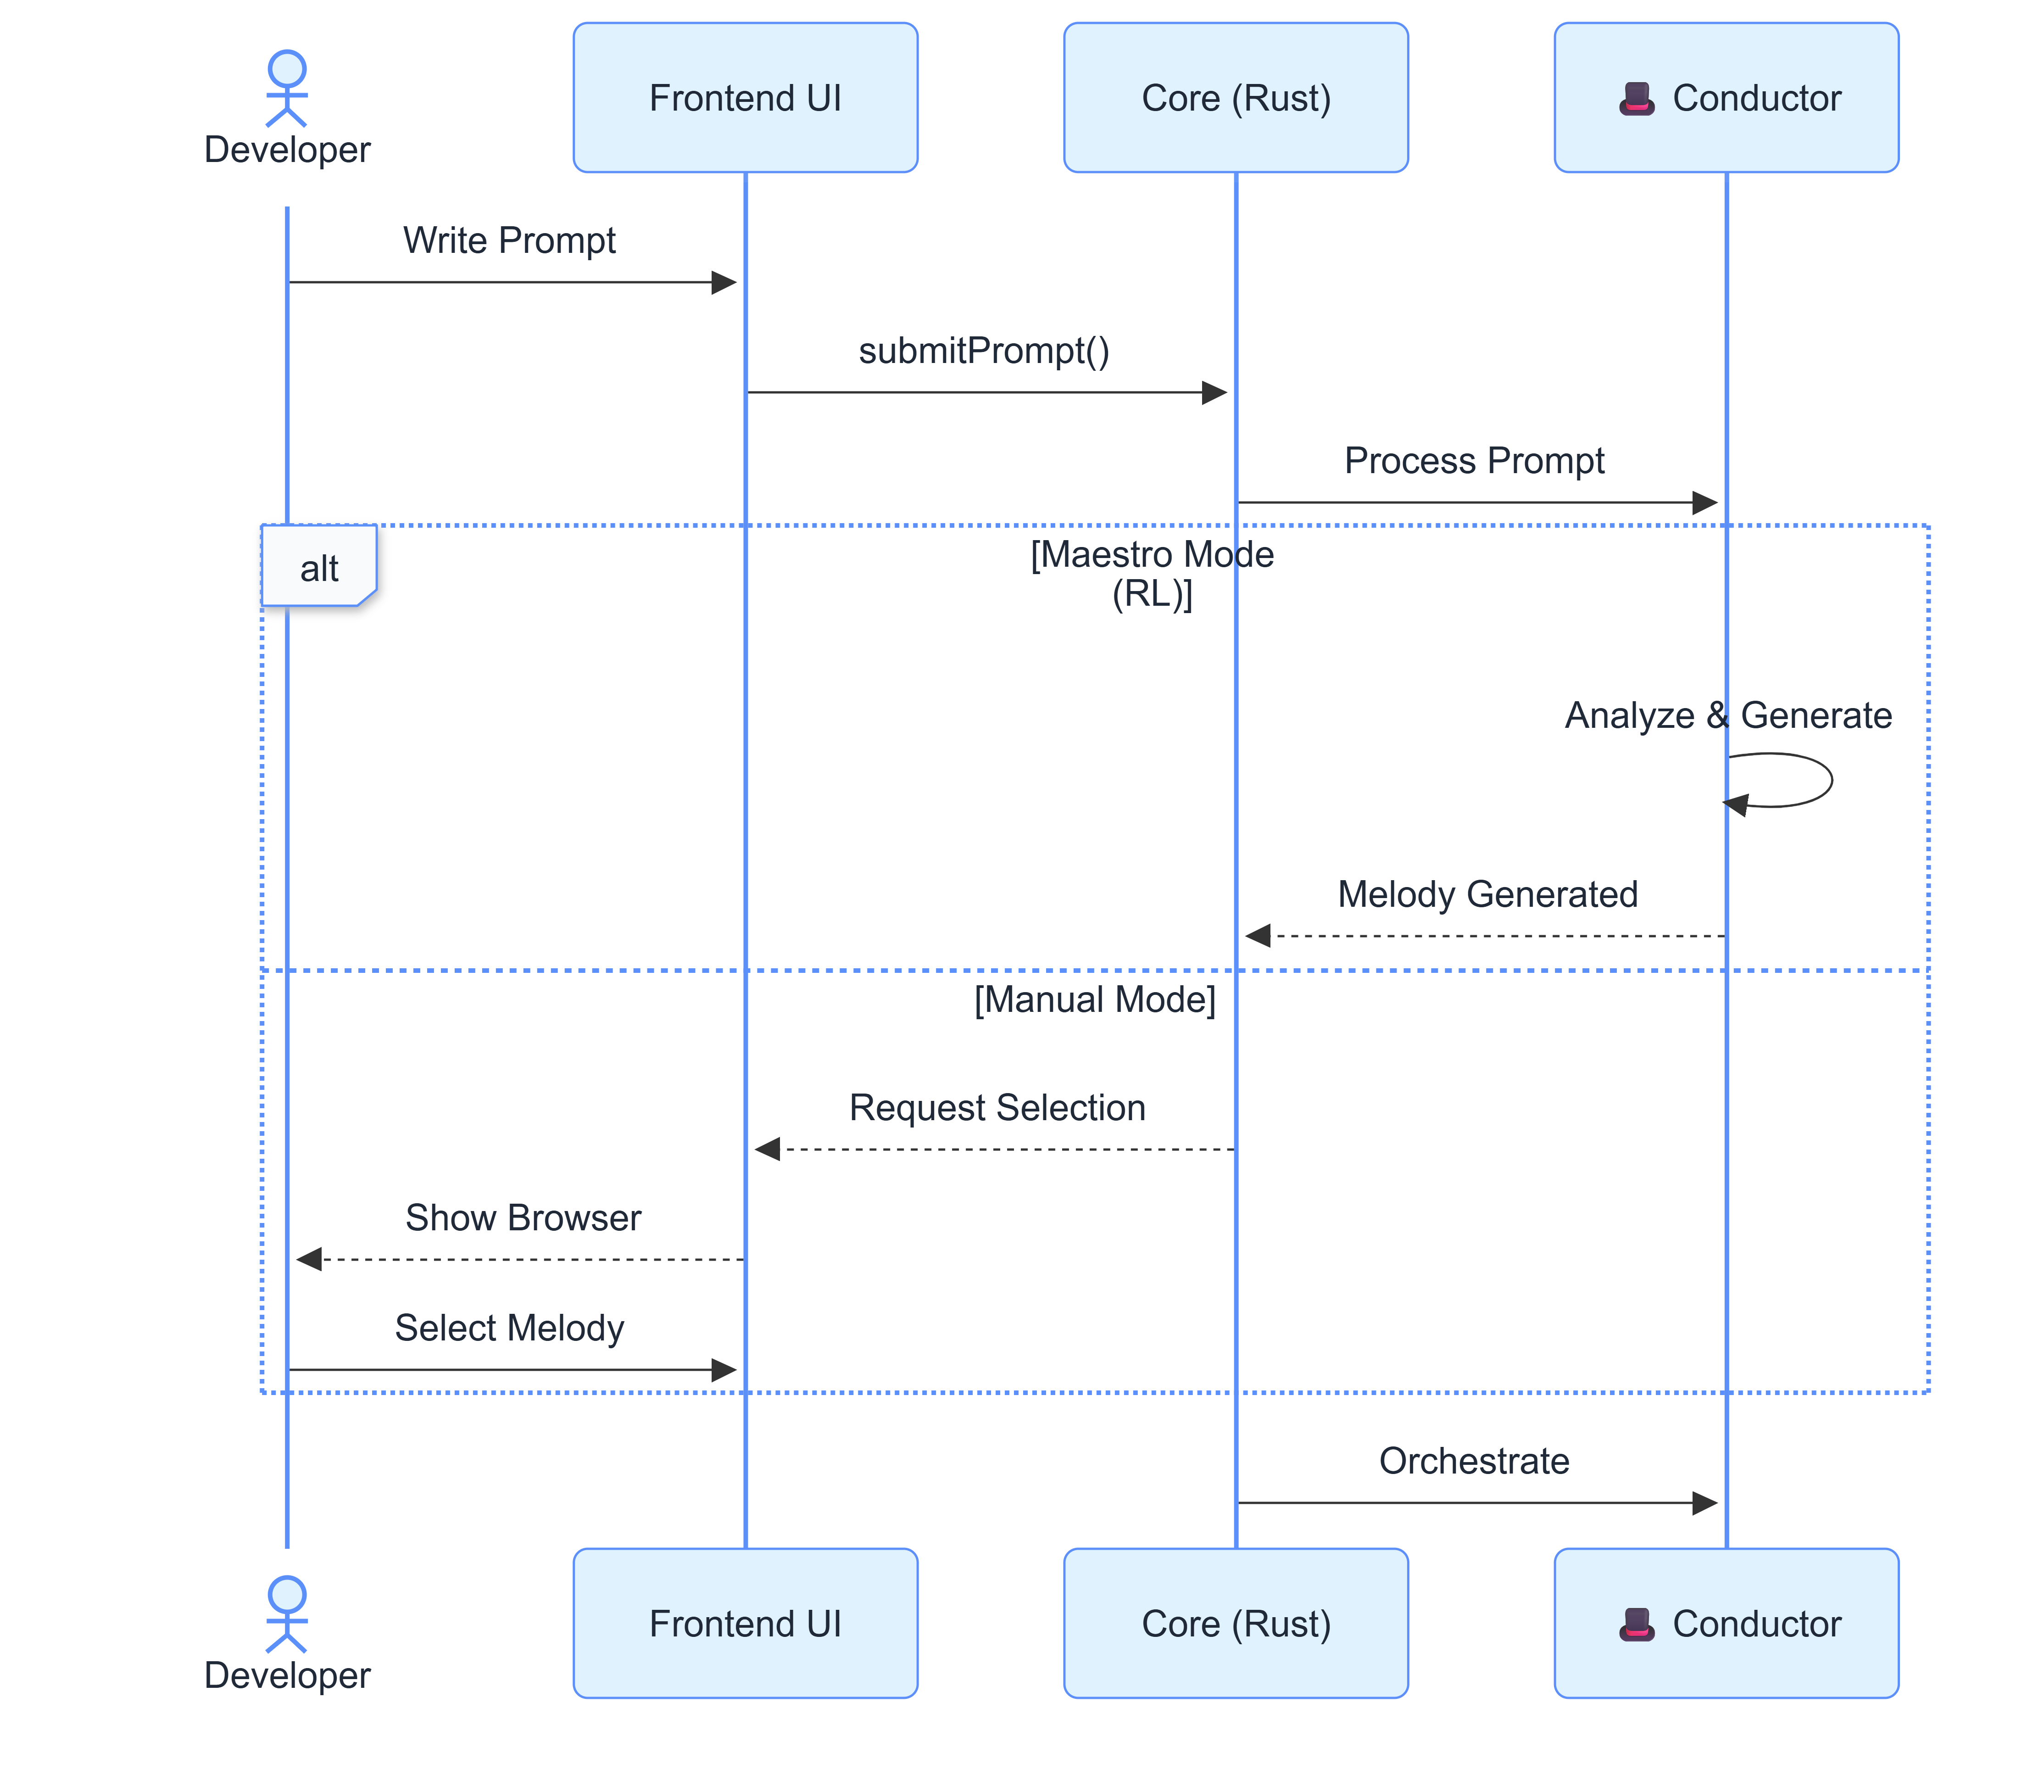
\includegraphics[width=0.95\textwidth]{images/diagrams/sequence_diagram/seperate_1_developer_workflow_execute_melody/Orchestration Flow.png}
\caption{Melody Orchestration Flow}
\label{fig:3.19-melody-orchestration}
\end{figure}

\clearpage
\textbf{Phase 2: Execution Flow}

After orchestration, the Conductor dispatches tasks to The Pit for execution. The Pit coordinates with the Pool Manager to allocate Player extensions, ensuring required AI models and tools are ready. The DAG Tracker manages task execution order based on dependencies, running each task in sequence or parallel as appropriate. As tasks complete, their results are stored in the ArtifactStore with unique identifiers. The Pit monitors execution progress and handles any errors that occur during task processing as illustrated in ~\ref{fig:3.20-melody-execution}.

\begin{figure}[H]
\centering
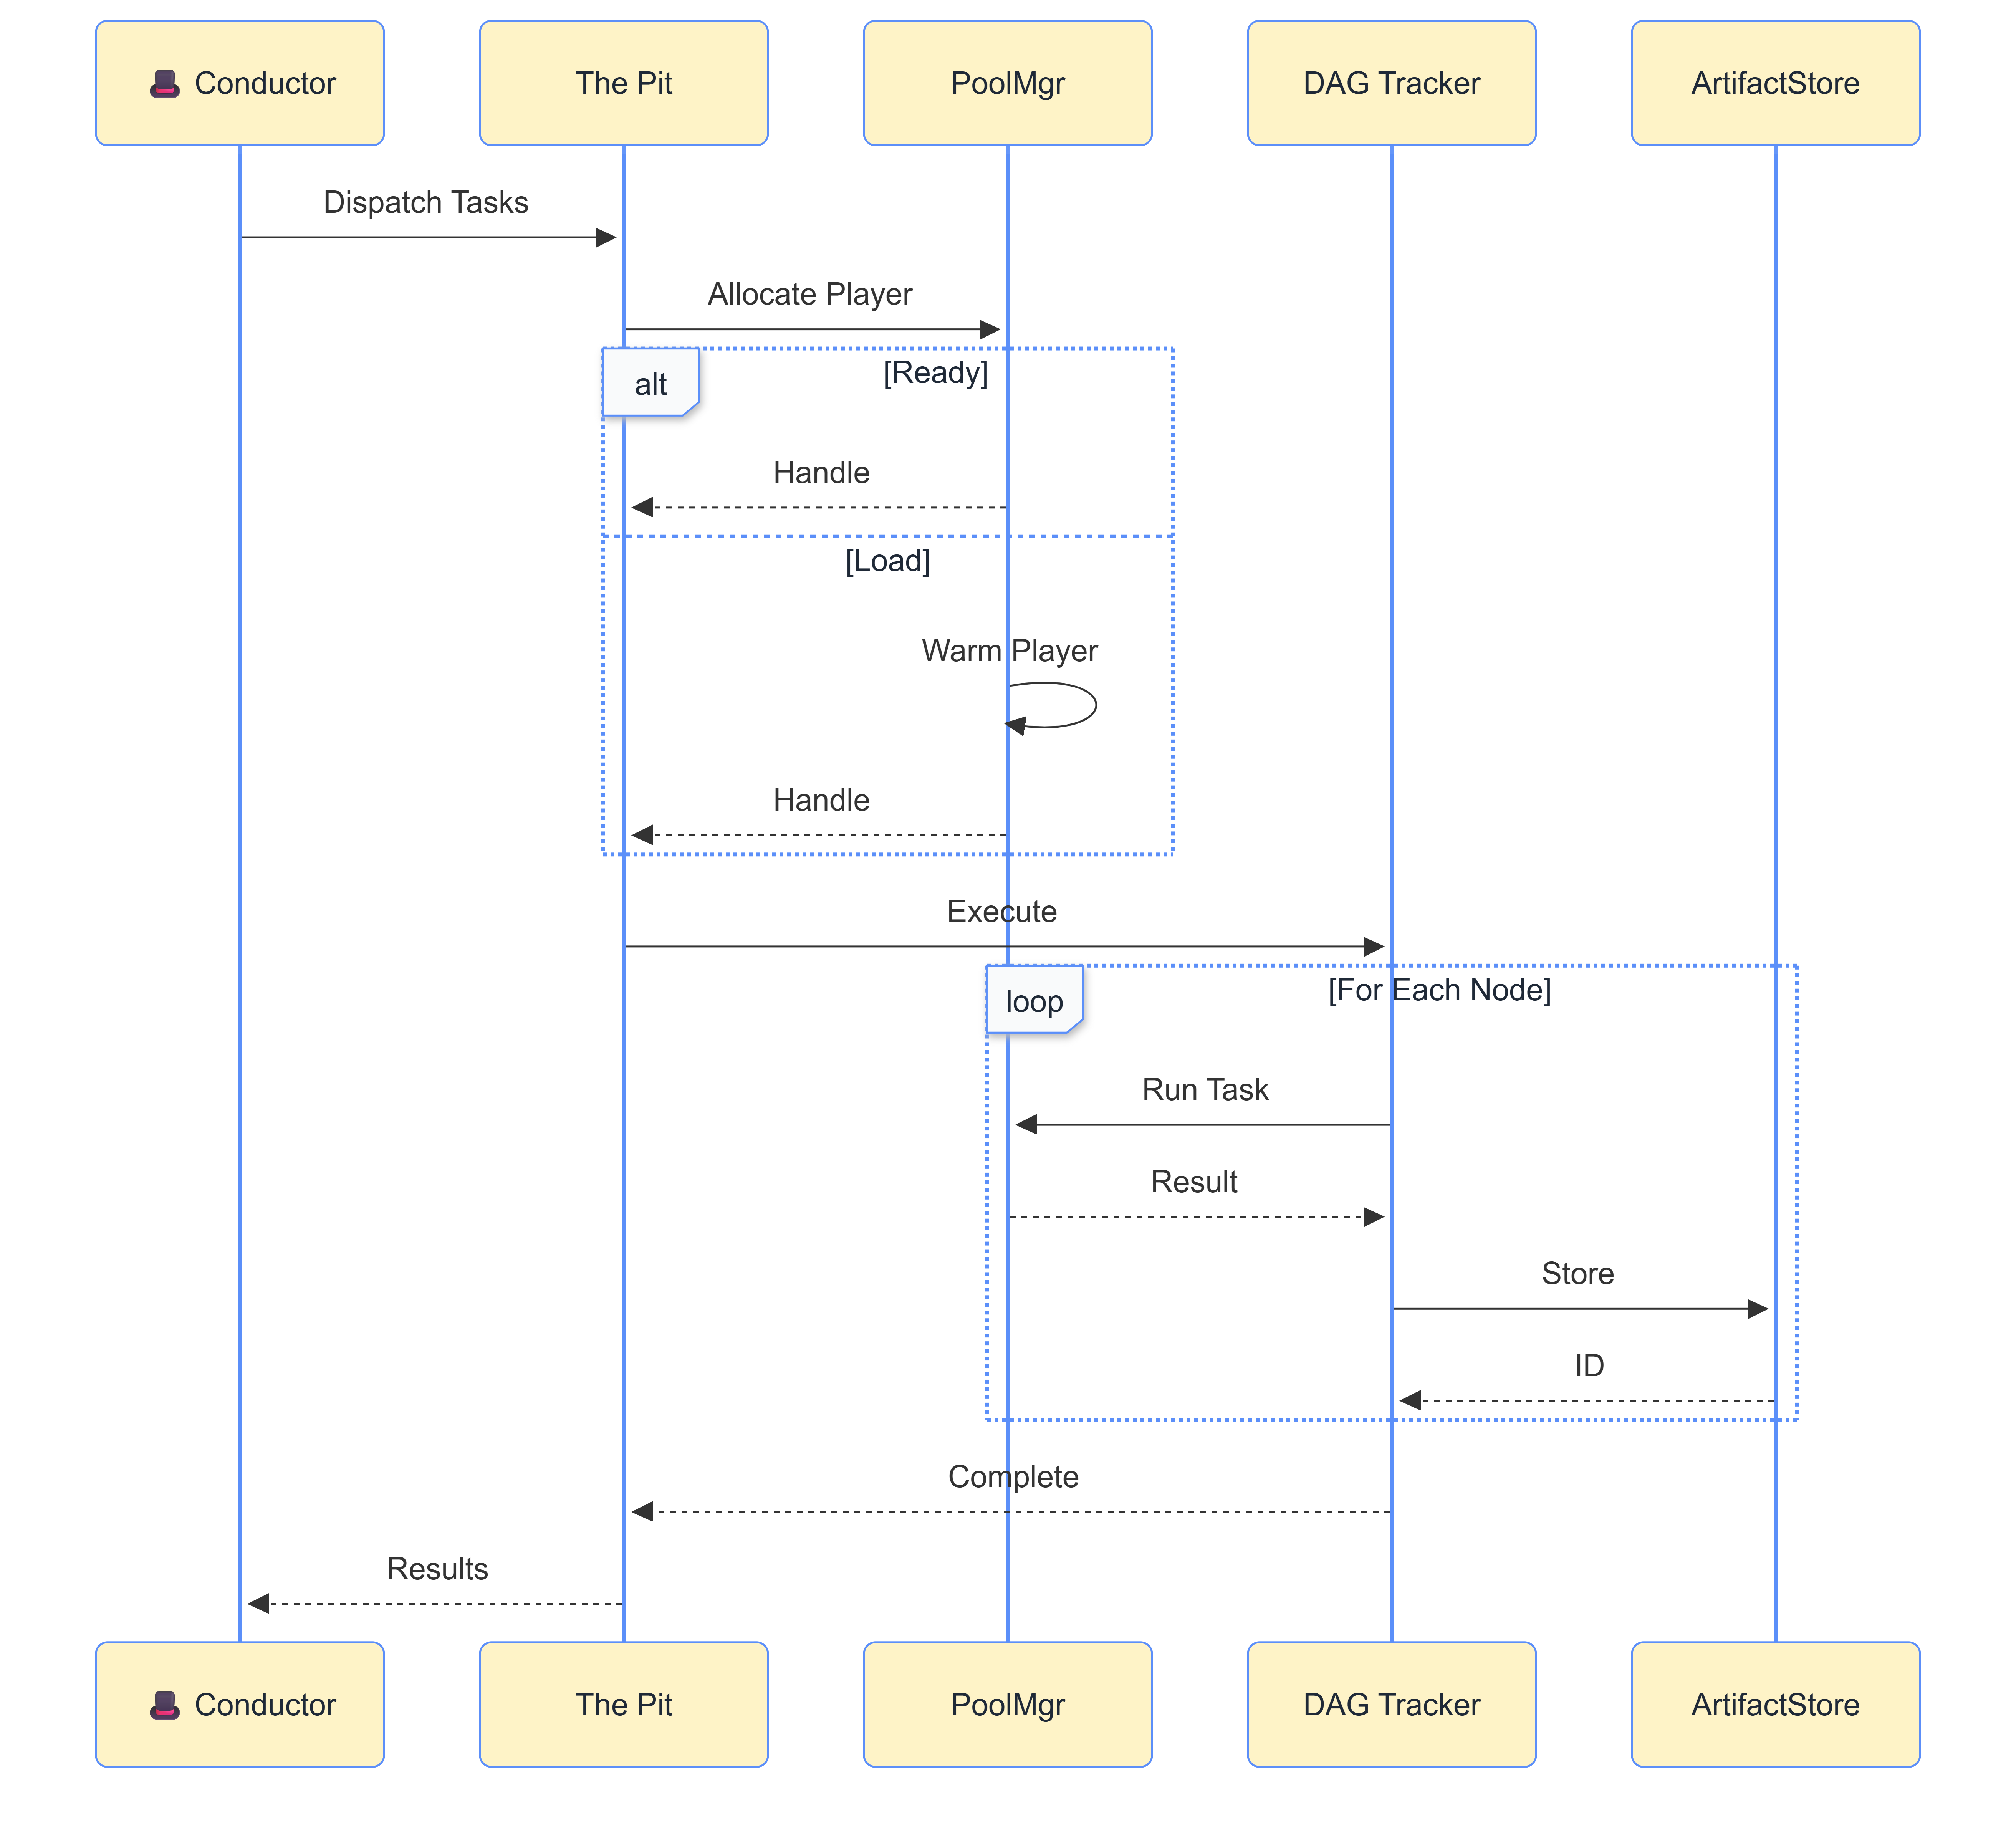
\includegraphics[width=0.95\textwidth]{images/diagrams/sequence_diagram/seperate_1_developer_workflow_execute_melody/Execution Flow.png}
\caption{Melody Execution Flow}
\label{fig:3.20-melody-execution}
\end{figure}

\clearpage
\textbf{Phase 3: Data Retrieval Flow}

Once execution completes, the Core system sends status updates to the Frontend UI, which displays results to the developer. When the developer requests to view artifacts, the UI queries the Core system, which retrieves data from the ArtifactStore. The stored artifacts are returned through the system layers and displayed to the developer. This completes the full Melody execution cycle, with the Conductor calculating rewards and updating its model to improve future workflow generation as illustrated in ~\ref{fig:3.21-melody-retrieval}.

\begin{figure}[H]
\centering
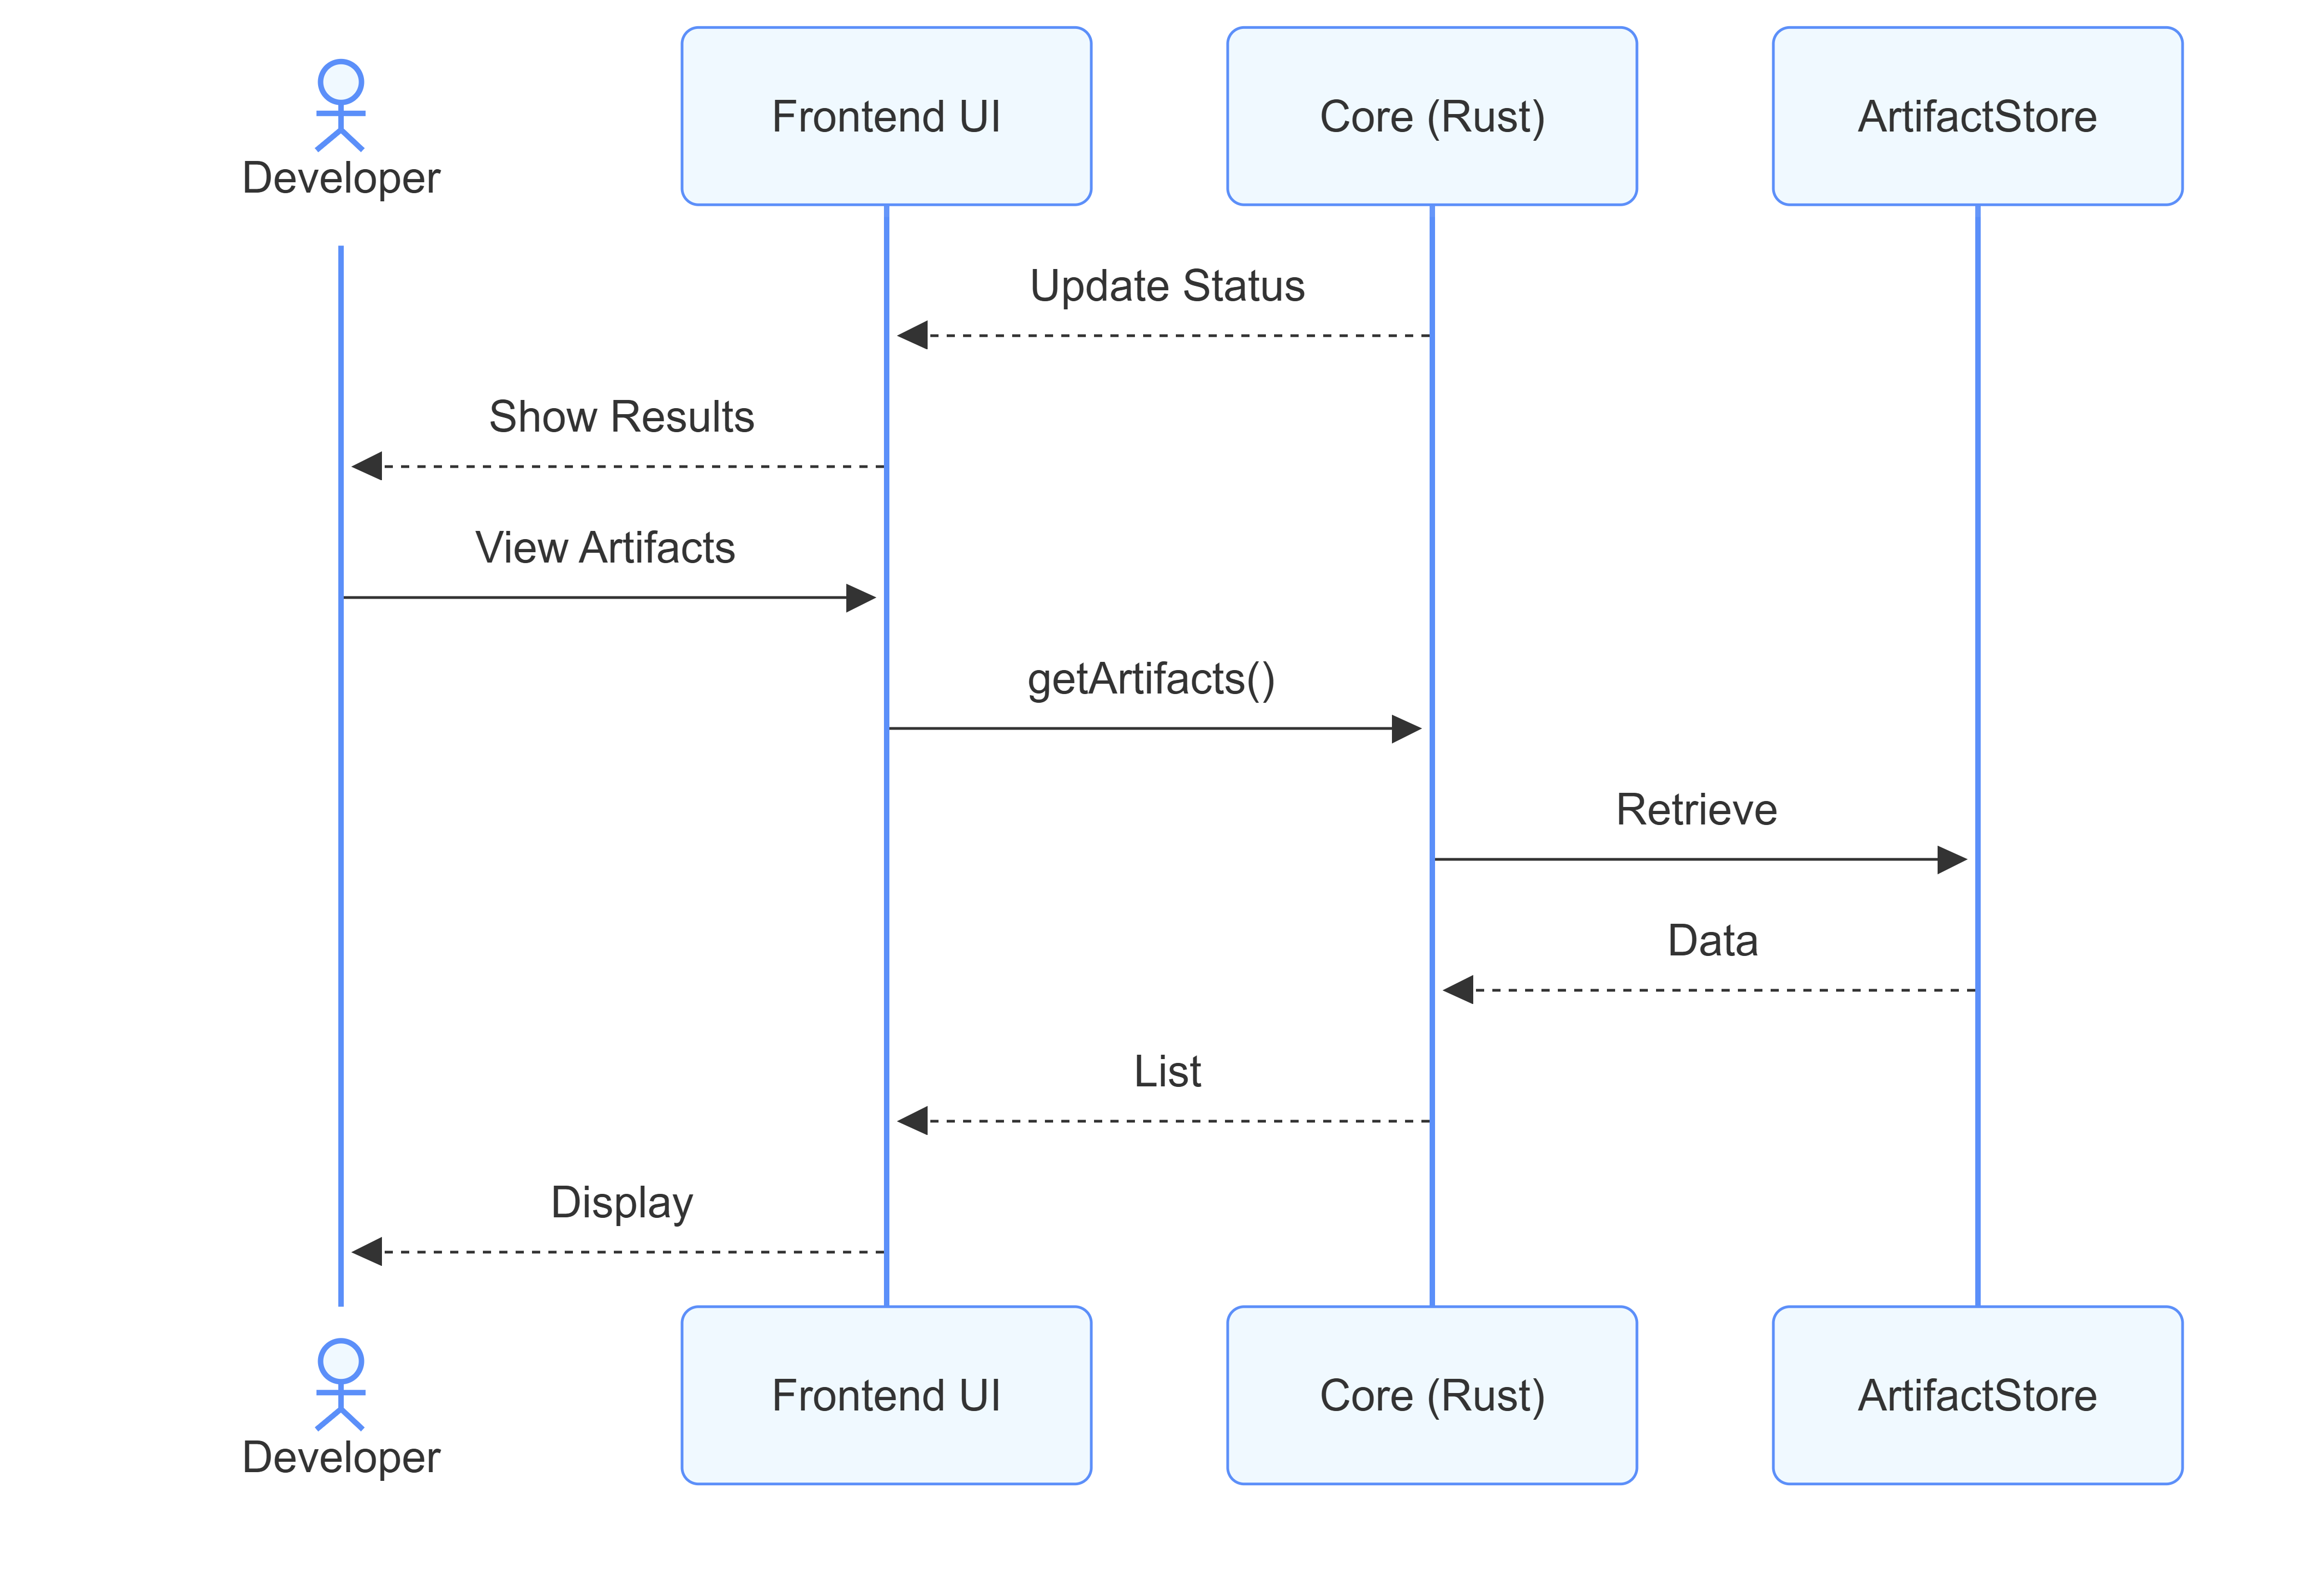
\includegraphics[width=0.95\textwidth]{images/diagrams/sequence_diagram/seperate_1_developer_workflow_execute_melody/Data Retrieval Flow.png}
\caption{Melody Data Retrieval Flow}
\label{fig:3.21-melody-retrieval}
\end{figure}

\clearpage

The workflow generation process implemented by the Conductor involves several sophisticated steps that transform a natural language prompt into an executable workflow, which can be understood through two main phases:

\textbf{Phase 1: Inference \& Generation}

The process begins with intent parsing, where the Conductor receives a complex prompt from the developer through the Frontend UI and Core system. The Conductor analyzes the prompt using natural language understanding techniques to extract key objectives, constraints, and preferences. It then queries the RL Model to get action probabilities through a forward pass. The RL Model generates an action distribution that guides workflow construction. The Conductor uses these probabilities to generate the workflow structure, with the Melody Engine creating a concrete workflow graph where nodes represent extension invocations and edges represent data dependencies. The generated Melody is then previewed to the developer through the UI, displaying the workflow graph for review before execution as illustrated in ~\ref{fig:3.22-conductor-inference}.

\begin{figure}[H]
\centering
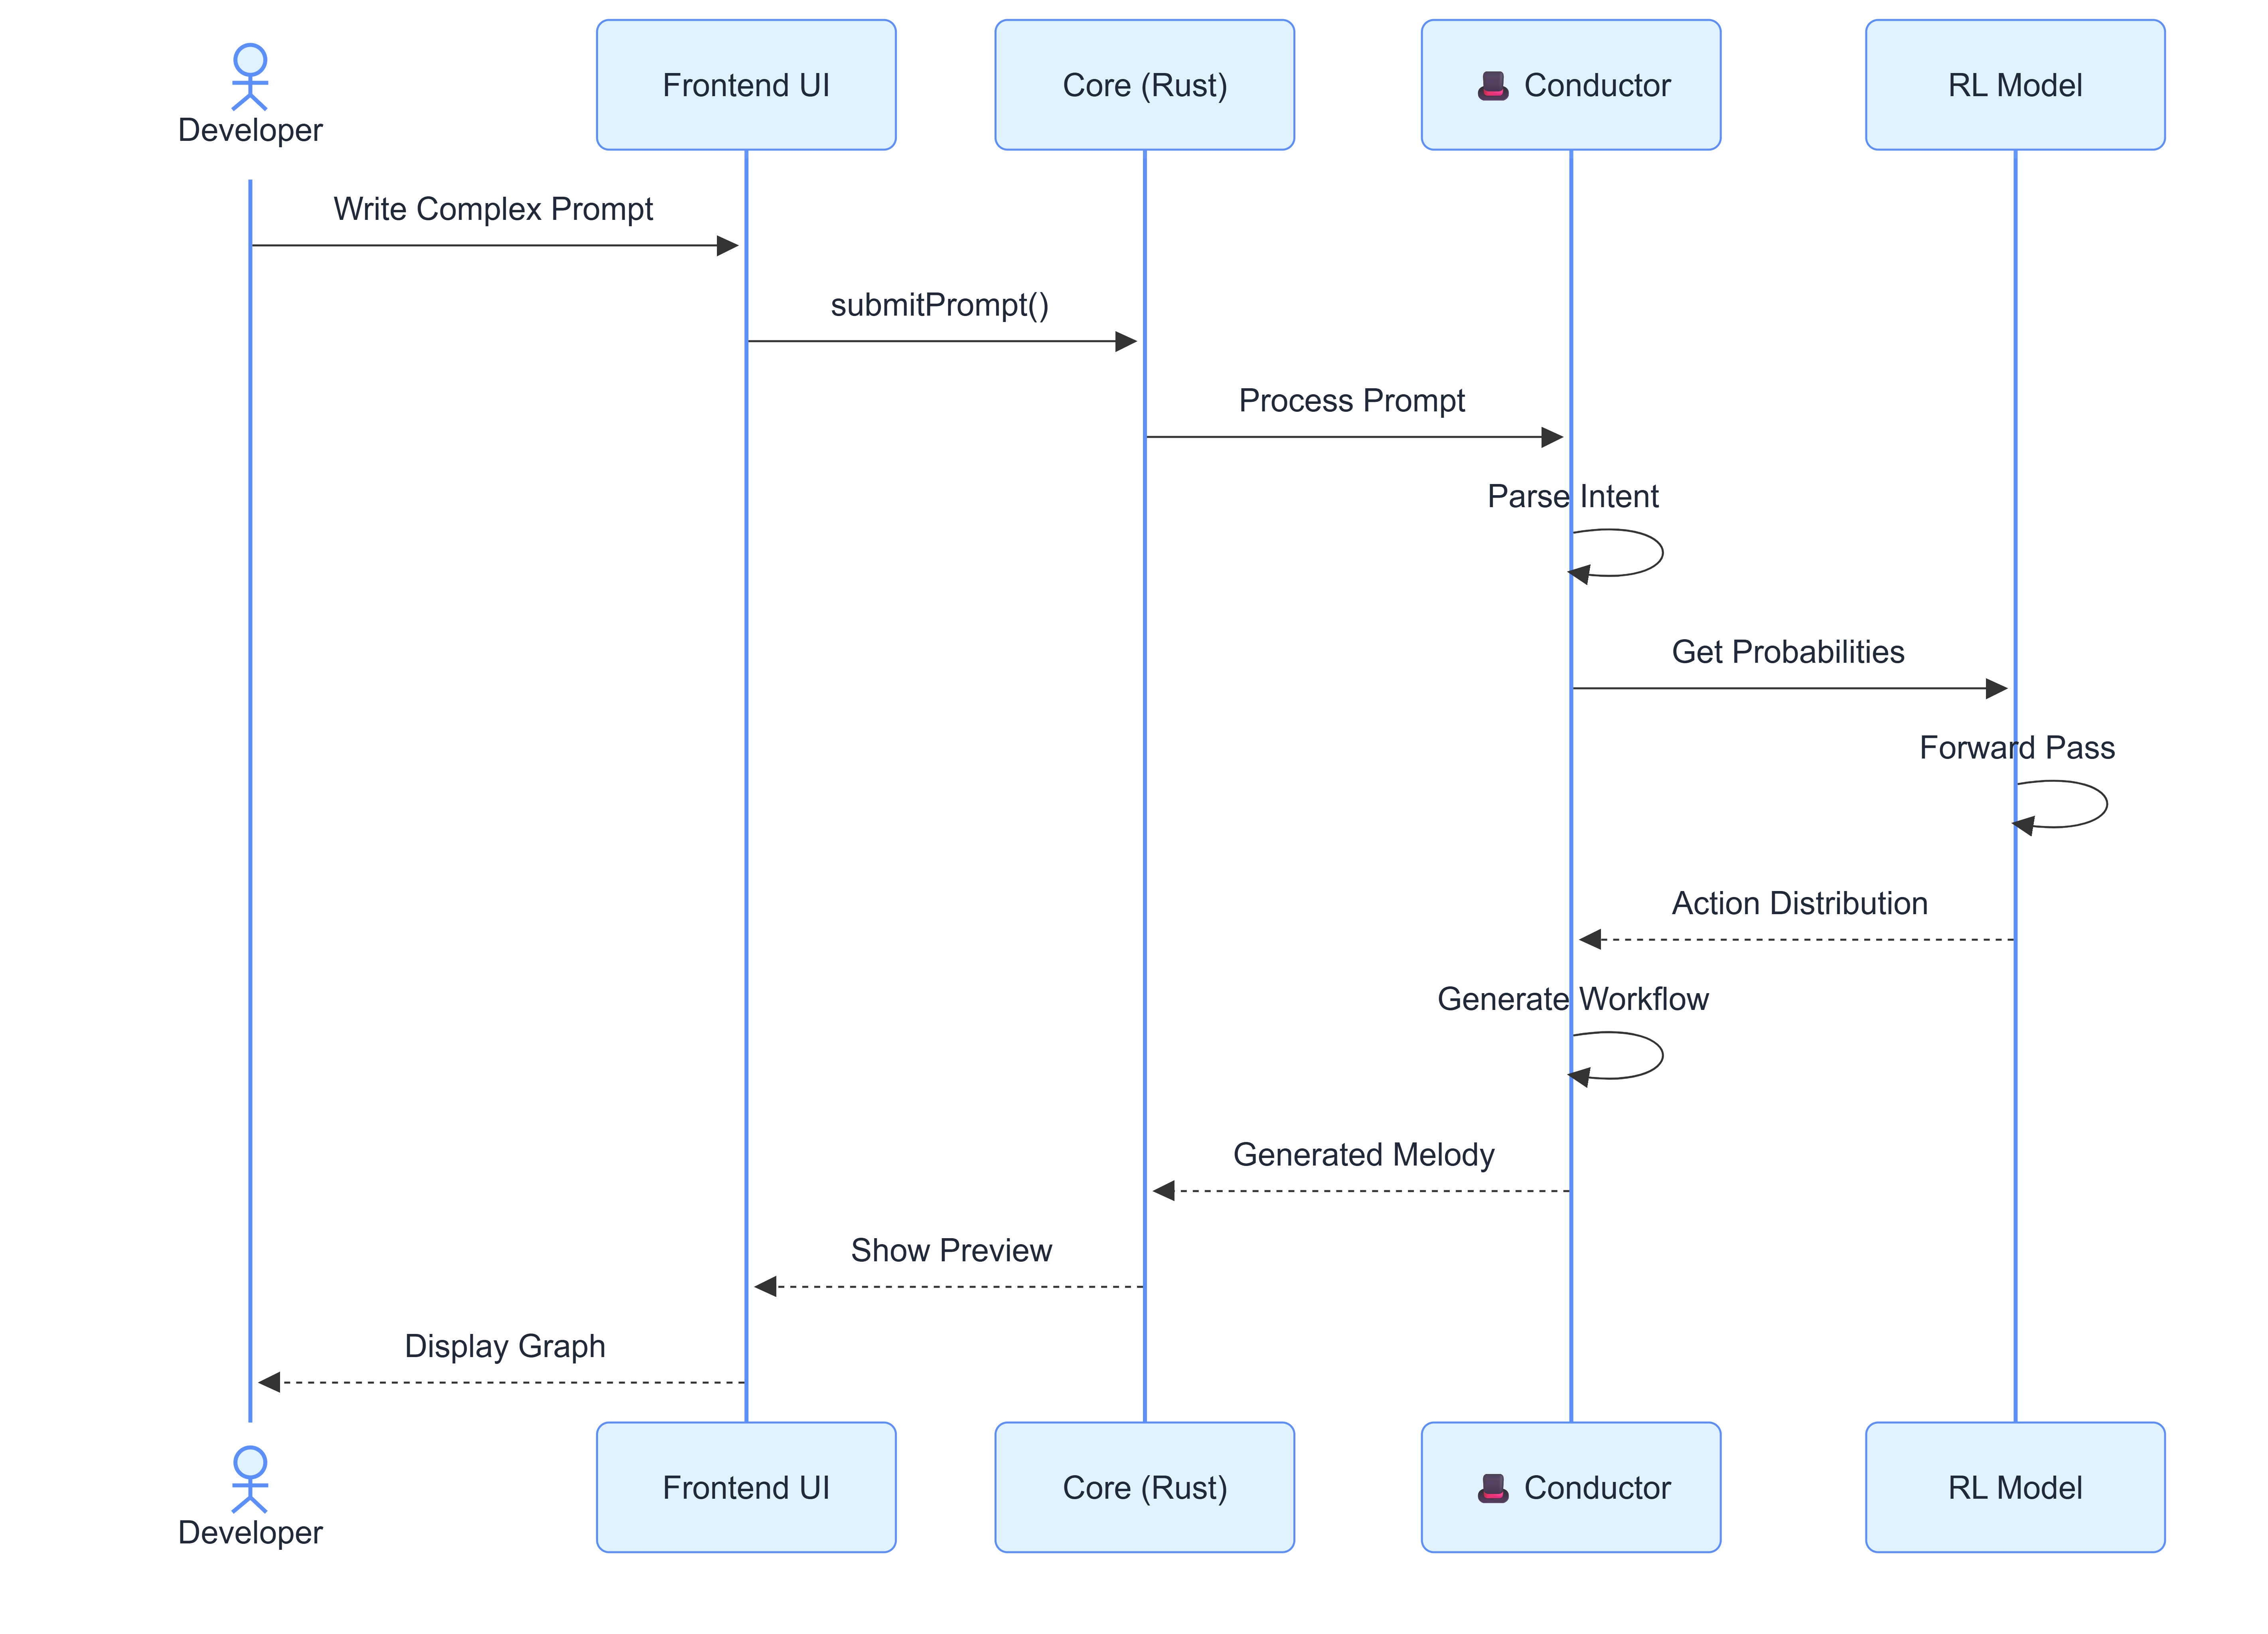
\includegraphics[width=0.95\textwidth]{images/diagrams/sequence_diagram/seperate_4_conductor_workflow_generate_melody/Inference & Generation.png}
\caption{Conductor Inference \& Generation Phase}
\label{fig:3.22-conductor-inference}
\end{figure}

\clearpage
\textbf{Phase 2: Execution \& Learning}

After the developer approves and executes the Melody, the Core system starts execution and the Conductor dispatches tasks to the Bridge component. During execution, the Conductor collects execution metrics including success rates, execution time, and artifact quality. These metrics are used to update the RL Model through backpropagation, implementing the reinforcement learning cycle where the model learns from experience. The RL Model calculates rewards based on the execution outcome (State → Action → Reward) and updates its parameters to improve future workflow generation. Optionally, the developer can save the successful Melody to the Polyphony marketplace, making it available for reuse by other developers. This continuous learning cycle enables the Conductor to improve its workflow generation capabilities over time as illustrated in ~\ref{fig:3.23-conductor-learning}.

\begin{figure}[H]
\centering
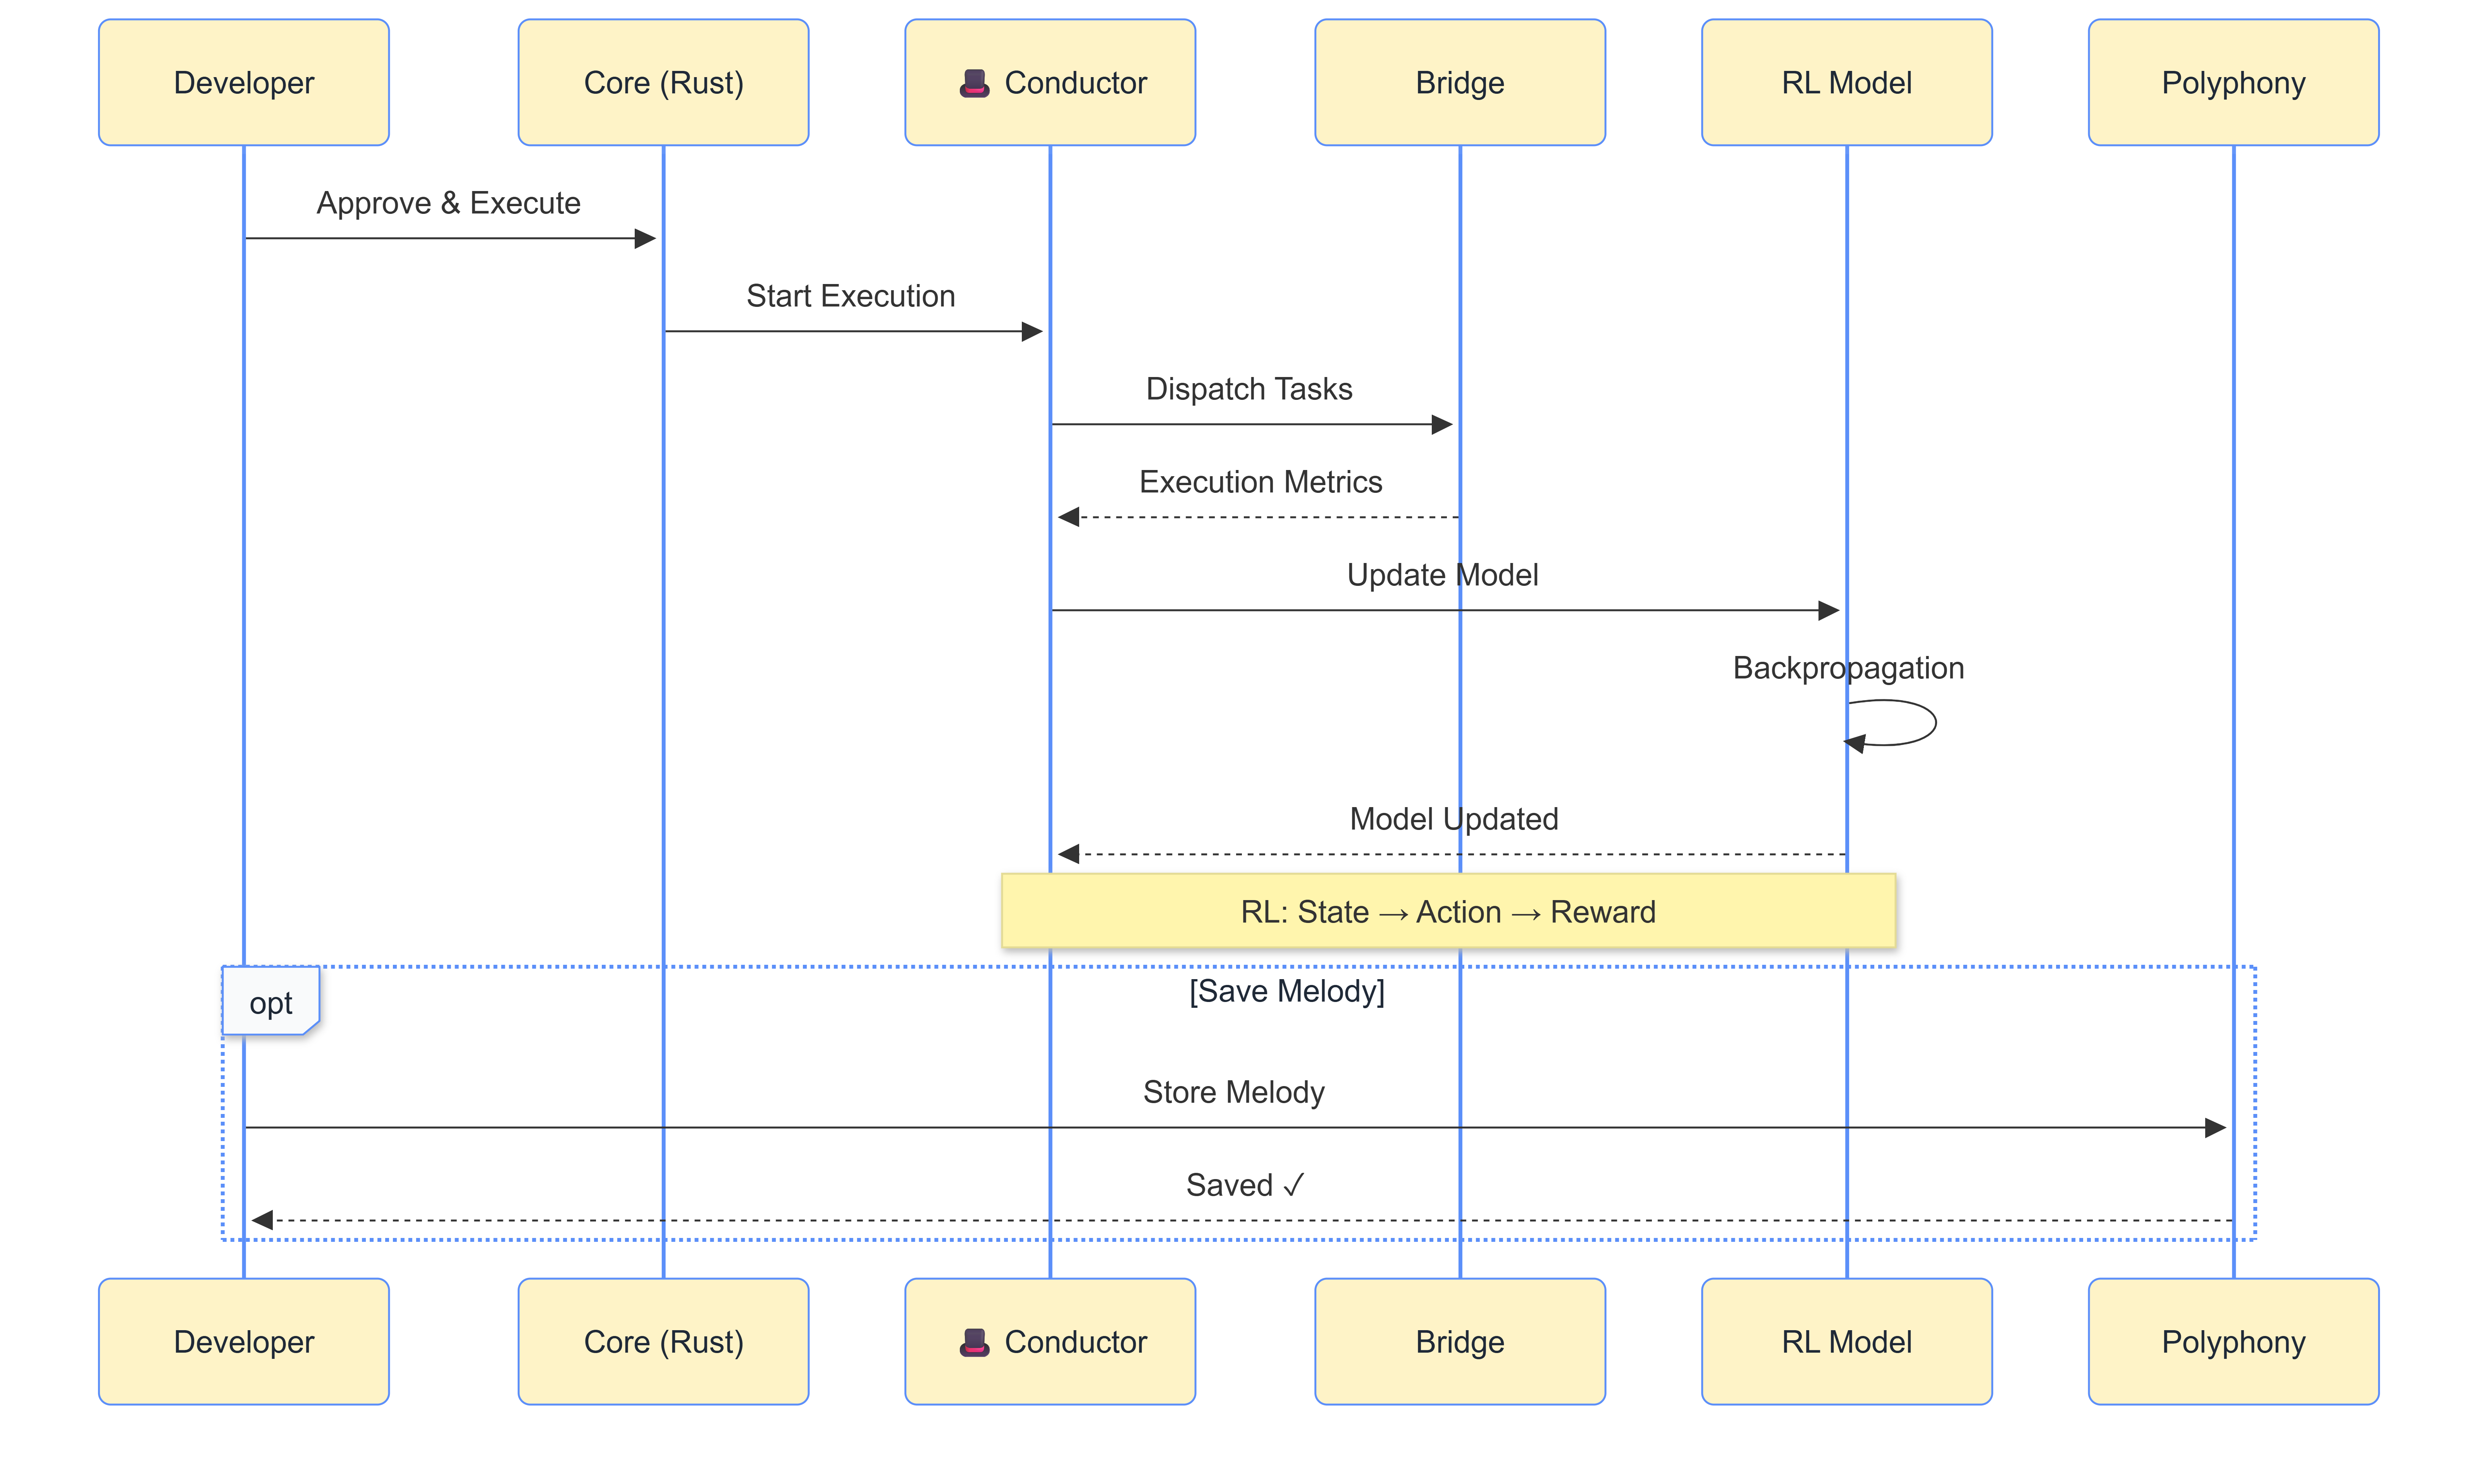
\includegraphics[width=0.95\textwidth]{images/diagrams/sequence_diagram/seperate_4_conductor_workflow_generate_melody/Execution & Learning.png}
\caption{Conductor Execution \& Learning Phase}
\label{fig:3.23-conductor-learning}
\end{figure}

% \clearpage
\subsection*{3.8.3 Workflow Execution and Validation}
\addcontentsline{toc}{subsection}{3.8.3 Workflow Execution and Validation}

The Melody execution lifecycle follows a well-defined state machine governing progression from workflow creation through completion as illustrated in ~\ref{fig:3.24-melody-states}. Melodies begin in the Draft state during composition, move through Validating for correctness checks (cycle detection, type safety, resource constraints), then Ready when validation passes. During execution, Melodies progress through Queued (waiting for resources), Executing (active processing), and optionally Paused (for checkpointing or intervention), concluding in either Completed or Failed states.

\begin{figure}[H]
\centering
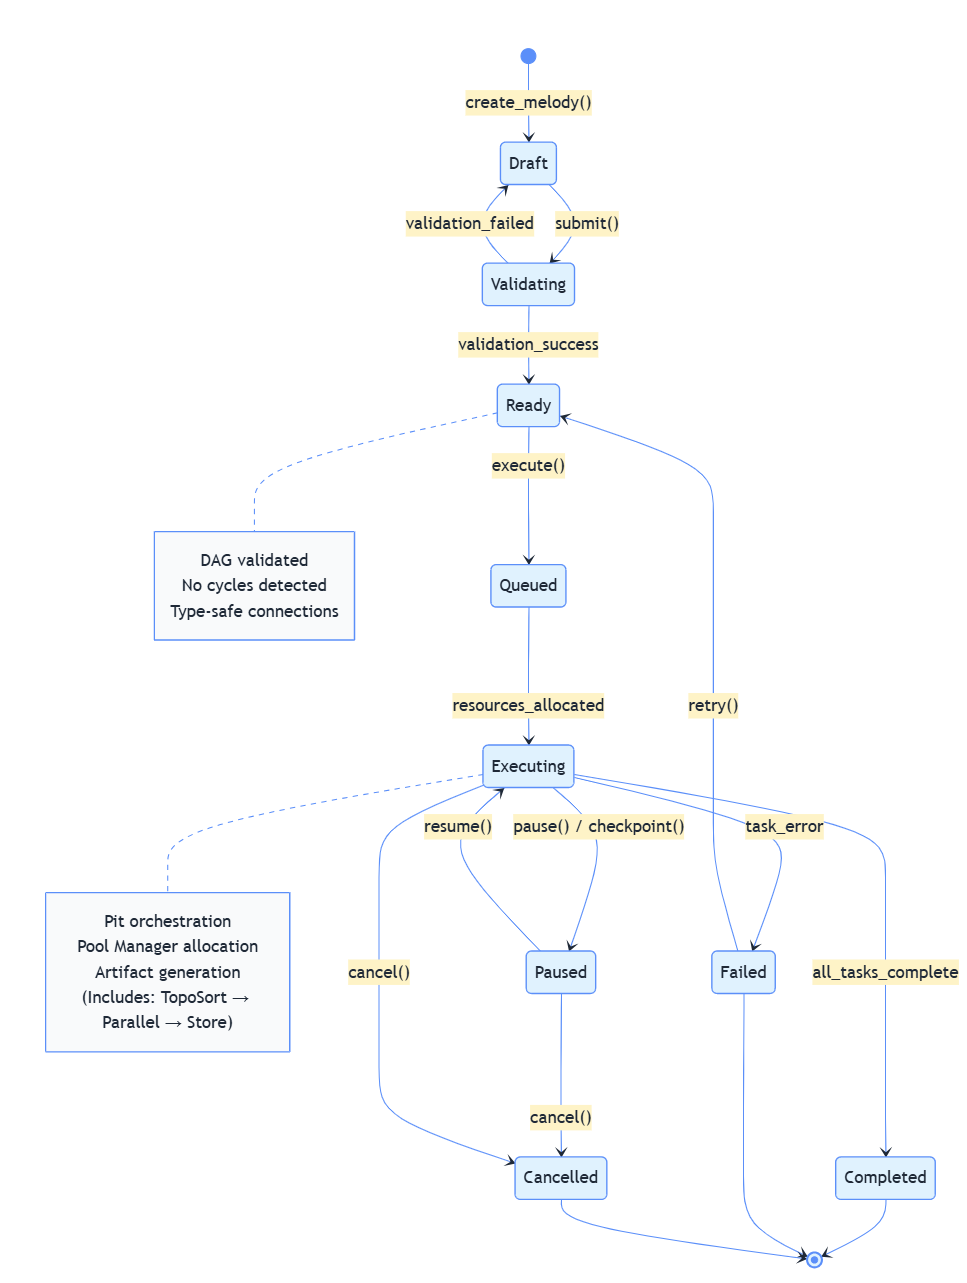
\includegraphics[width=1.05\textwidth]{images/diagrams/state_diagram/3_melody_execution_workflow.png}
\caption{Melody Execution State Machine}
\label{fig:3.24-melody-states}
\end{figure}

The orchestration system supports multiple execution modes: Maestro Mode for fully automated workflow generation from natural language prompts, Manual Mode for browsing and selecting pre-built Melodies from the Polyphony Store, and Hybrid approaches combining automated generation with manual refinement.

The workflow validation process ensures correctness before execution through cycle detection (ensuring acyclic graphs), type safety verification (compatible data flow), resource constraint validation (available resources), and dependency resolution (installed extensions). The DAG Tracker enables parallel execution by identifying independent tasks that can run concurrently, maximizing computational resource utilization while managing allocation and error handling.

Checkpoint and resume capabilities enable long-running workflows to survive system restarts by periodically saving execution state (completed tasks, outputs, remaining work). If interrupted, the system resumes from the most recent checkpoint, re-executing only incomplete tasks.

The Agent-Driven Development paradigm enabled by the orchestration system represents a fundamental shift where developers provide high-level intent while AI agents handle implementation details. This reduces cognitive load, increases productivity through automation, improves consistency by applying proven patterns, and enables exploration of different approaches.

